% !TeX root=../main.tex

\section{Probabilistic Trace Alignment Pipeline}
We now provide a technique for computing probabilistic trace alignments. Our approach takes as input
\begin{inparaenum}[\it (i)]
\item a reference model represented as aTG $\tg$,
\item a minimum, positive probability threshold $\pmin \in (0,1]$
\item a trace $\trace$ of interest,
\end{inparaenum}
and returns a ranking over all the $\net$-traces having a probability at least $\pmin$, based on a combination of their probabilities
(probabilistic component) and their distance to $\trace$ (alignment component).


\subsection{Computation pipeline}
We follow the pipeline shown in \figurename~\ref{fig:pipe} and described next.
%
\begin{figure}[!t]
	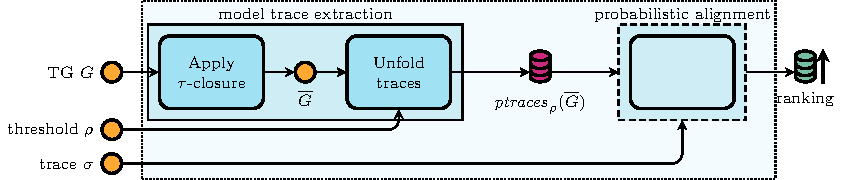
\includegraphics[width=\columnwidth]{images/pipelineShort}
	\caption{Pipeline to assess the probabilistic trace alignment.}\label{fig:pipe}
\end{figure}
%
%
%In step 1, the reachability graph $\rg{\net}$ of $\net$ is constructed.
%%
%In step 2,  $\rg{\net}$ is converted into a corresponding transition graph $\tg_{\rg{\net}}$ that preserves model traces and their
%probabilities. We omit the details of this conversion, due to lack of space and the fact that it employs well-known techniques used
%to \emph{shift labels} from transitions to states while preserving the behavior encoded by a transition system.
%\figurename~\ref{fig:orig} shows the result of this conversion when applied to the reachability graph in \figurename~\ref{fig:rg}.
%
The original TG $\tg$ is processed through a \emph{$\hidden$-closure} that compiles away all invisible transitions, resulting in
a new TG $\closed{\tg}$ using $\hidden$ labels only in the initial and accepting states, without modifying the
model traces or their probabilities. We omit the details, which rely on well-known automata-based techniques for removing
$\epsilon$-moves. The only observation is that, to preserve probabilities, we assume that the TG has no $\tau$ loops with
positive probability. In other words, we assume that all possible movements are observable.
The TG in \figurename~\ref{fig:lmc} already has this shape.

The next step unfolds the TG $\closed{\tg}$ to collect all the traces with probability at least $\pmin$. For this, we rely on a key
property of loops. Since the probability of a path is the product of the probabilities of the transitions, a loop can only have
probability 1 if all its transitions have probability 1 themselves. Assuming no periodic behavior appears, an execution of a
loop must decrease the probability. Thus, all valid sequences with a resulting probability of at least $\pmin$ can be enumerated.
These sequences are merged by trace, summing up their probabilities, thus obtaining the set $\ptraces{\closed{\tg}}{\pmin}$
of all the traces having a probability at least $\pmin$. The closure operation ensures that the notion of model trace collapses to
that of run modulo removing the initial and the final $\tau$ labels attached to the initial and accepting nodes.

The last step ranks the model traces considering their probabilities and the similarity with the input trace $\trace$. In
\figurename~\ref{fig:pipe}, this is shown as a black-box. We implement this last step in two alternative ways: one
computationally demanding but guaranteeing an optimal ranking, the other more efficient but yielding approximate ranking without
optimality guarantees.

\endinput

%%%%%%%%%%%%%%%%%%%%
%%%%%%%%%%%%%%%%%%%%
%%% END INPUT
%%%%%%%%%%%%%%%%%%%%
%%%%%%%%%%%%%%%%%%%%

%
We can show that the TG obtained in Definition \ref{def:transf} preserves the same set of probabilistic traces associated by the reachability graph. The proof is omitted due to the lack of space.

\begin{example}
\figurename~\ref{fig:lmc} shows the TG obtained from the reachability graph in \figurename~\ref{fig:rg}. Nodes are labeled with the firing
transition labels (in green), and edges preserve the probabilistic information from the reachability graph (in red). Intuitively, when a
new initial node \textit{\textbf{i}} is inserted, we preserve all the initial probabilistic choices that a transition is fired from an initial
marking $M$, while the intermediate edges inherit the probabilistic choice of the firing transition from the subsequent choices. When
a new final node \textit{\textbf{f}} is added, such edges always have probability $1$, and thus do not interfere with the
initial traces' probability.
\end{example}

\subsection{$\tau$-closure}\label{sec:clos}
The $\tau$-closure process has two main purposes: first, reduce the size of the previously generated TG by removing all
$\tau$-labeled nodes \texttt{\color{blue}w} and preserving the connection between  the nodes \texttt{\color{blue}u}
from its ingoing edges   $\texttt{\color{blue}u}\xrightarrow{\color{violet}\rho}\texttt{\color{blue}w}$ with the nodes \texttt{\color{blue}v} from its ingoing edges   $\texttt{\color{blue}w}\xrightarrow{\color{violet}\rho'}\texttt{\color{blue}v}$ by establishing new edges $\texttt{\color{blue}u}\xrightarrow{\color{violet}\rho\rho'}\texttt{\color{blue}v}$. $\tau$-labeled initial (or accepting) nodes are removed iff they have only one outgoing (ingoing) edge with probability $1$.

\begin{example}\todo{Is it now ok?}
	The $\tau$-closure removes the non-initial and non-accepting nodes within an automaton, while preserving the probabilistic trace equivalence of the two automata. Let us suppose to apply the $\tau$-closure to the automata in \figurename~\ref{fig:orig}: node \texttt{\color{blue}10} is removed alongside its associated edges, and new edges $\texttt{\color{blue}3}\xrightarrow{\color{violet}\rho_{65}}\texttt{\color{blue}4}$ and $\texttt{\color{blue}3}\xrightarrow{\color{violet}\rho_{6f}}\texttt{\color{blue}5}$ are introduced. The resulting TG $P$ is represented with the same graphical depiction \figurename~\ref{fig:closed}.
\end{example}
%
Consequently, it is always possible to minimize a TG  via $\tau$-closure, so that the only nodes labeled as $\tau$
are the source and the target nodes and the set of weighted traces is preserved. From now on, we consider only minimized TGs.

\subsection{Unfolder}\label{sec:unrav}
%Being that both the graph isomorphism problem is NP-Complete and the
Since TGs are fully characterized by the set of the probabilistic traces that they generate,  we say that two TGs are
(probabilistic-trace) equivalent iff they share the same set of weighted traces. In particular, we denote as $\mathcal{W}_p^n(P)$ the set of all the weighted traces in $P$ having at least probability $p$ and maximum length $n$. Under these assumptions, the probabilistic trace equivalence is deterministic.

\begin{example}
	The set $\mathcal{W}_0^{\aleph_0}(P^*)$ of weighted traces of the TG in \figurename~\ref{fig:orig} is
%	The TG in \figurename~\ref{fig:orig} has the following set $\mathcal{W}_0^{\aleph_0}(P^*)$ of weighted traces:
$$\set{\braket{\underbrace{\color{green}a\dots a}_{n},{\color{violet}\pa\pc^n\pf}}|n\in \mathbb{N}_{>0}}\cup \set{\braket{{\color{green}c}\underbrace{\color{green}a\dots a}_{n},{\color{violet}\pb\pd\pc^n\pf}}|n\in \mathbb{N}_{>0}}\cup\{\braket{{\color{green}cb},{\color{violet}\pb\pe}}\}$$
After the $\tau$-closure process, $\mathcal{W}_0^{\aleph_0}(P^*)=\mathcal{W}_0^{\aleph_0}(P)$, so the two TGs are (probabilistic-trace) equivalent.
\end{example}
